% IEEE journal template, with the 10pt two-column format required by TWC.
% Compile from paper/TWC-2/; keep the IEEEtran fonts and page dimensions.
% Select T1 before the class selects Times, including under XeTeX/Tectonic.
\RequirePackage[T1]{fontenc}
\documentclass[10pt,journal,letterpaper]{IEEEtran}
\usepackage{amsmath,amssymb,bm,booktabs,array}
\usepackage{graphicx}
\usepackage{cite}
\usepackage{enumitem}
\usepackage{tikz}
\usetikzlibrary{arrows.meta,positioning}
\usepackage[hidelinks]{hyperref}
\graphicspath{{figures/}}
\interdisplaylinepenalty=2500

\newcommand{\CN}{\mathcal{CN}}
\newcommand{\E}{\mathbb{E}}
\newcommand{\I}{\mathbf{I}}
\newcommand{\vect}{\operatorname{vec}}
\newcommand{\tr}{\operatorname{tr}}
\newcommand{\diag}{\operatorname{diag}}
\newcommand{\logit}{\operatorname{logit}}
\newcommand{\sigmoid}{\operatorname{sigmoid}}
\newcommand{\clip}{\operatorname{clip}}
\newcommand{\relu}{\operatorname{Re}}
\newcommand{\imag}{\operatorname{Im}}
\newcommand{\norm}[1]{\left\lVert#1\right\rVert}

\title{Generative-Model-Aided Grant-Free Random Access for GNSS-Independent MIMO-AFDM Satellite IoT Systems}
% Author order and IEEE membership grades supplied by the author.
\author{Bo~Wang,~\IEEEmembership{Student~Member,~IEEE,}
Wenpeng~Jing,~\IEEEmembership{Senior~Member,~IEEE,}
Zhiqun~Hu,~\IEEEmembership{Senior~Member,~IEEE,}
Shirui~Zuo,~\IEEEmembership{Student~Member,~IEEE,}
and~Changhao~Liu,~\IEEEmembership{Student~Member,~IEEE}%
\thanks{All authors are with Beijing University of Posts and
Telecommunications (e-mails: wangb@bupt.edu.cn;
[Wenpeng Jing: e-mail to be added]; [Zhiqun Hu: e-mail to be added];
[Shirui Zuo: e-mail to be added]; [Changhao Liu: e-mail to be added]).}}

\begin{document}
\maketitle
\begin{abstract}
This paper investigates joint activity detection and channel estimation
(JADCE) for grant-free random access in low Earth orbit satellite
Internet-of-Things systems without global navigation satellite system
(GNSS) assistance. Large differential delays and Doppler shifts
complicate the pilot observation model, while fractional offsets weaken
sparse channel representations. We propose a multi-frame affine frequency
division multiplexing (AFDM) transmission scheme and derive its
input--output relationship, which retains the prefix phase for delays
beyond the useful symbol interval and separates the Doppler-induced
phase evolution across frames, yielding multiple observations of a
shared effective channel. A score-based generative prior is then
learned from multiantenna AFDM effective-channel samples generated with
continuous delays and Doppler shifts, thereby representing off-grid
effects and dependence among channel coefficients without a prescribed
sparsity pattern. From the posterior factorization, we develop a
deep-unfolded message-passing receiver that combines linear estimation
with channel and activity denoising. As activity probabilities weight
the channel estimates used in subsequent messages, we jointly train
the channel denoisers, activity classifiers, and message parameters
from received pilots, using score pretraining for initialization and
progressive training to adapt the updates to each layer's inputs.
\end{abstract}
% Numerical findings will be added after evaluation of the new receiver.
\begin{IEEEkeywords}
Affine frequency division multiplexing, satellite Internet of Things,
grant-free random access, joint activity detection and channel estimation,
score-based generative models, deep unfolding.
\end{IEEEkeywords}

\section{Introduction}
\label{sec:introduction}

Low Earth orbit (LEO) satellites extend Internet-of-Things (IoT)
services to remote areas, where grant-free random access (GFRA) can
reduce signaling overhead by allowing active devices to transmit
without first obtaining a grant. Since device activities are unknown
and limited pilot resources preclude mutually orthogonal pilots,
the receiver must perform joint activity detection and channel
estimation (JADCE) \cite{liu2018}, which is further complicated by
large propagation delays and Doppler shifts in LEO links.

The new radio non-terrestrial network (NR-NTN) framework in Release~17
of the 3rd Generation Partnership Project (3GPP) uses position information
from a global navigation satellite system (GNSS) receiver, satellite
ephemeris, and a broadcast common timing advance for uplink delay and
Doppler pre-compensation \cite{3gpp38300}. To support devices without
GNSS receivers or access to GNSS services, Release~19 includes a study
of GNSS-independent operation \cite{3gpp22865}. Handling differential
delays and Doppler shifts at the satellite reduces the GNSS hardware
and pre-compensation burden on IoT devices, but these offsets can
exceed one symbol duration and one subcarrier spacing, respectively.
Consequently, terrestrial orthogonal frequency division multiplexing
(OFDM)-based GFRA schemes designed for small offsets and block-fading
channels cannot be directly applied.

Waveforms for doubly selective channels offer a starting point:
orthogonal time-frequency space (OTFS) modulation exploits diversity
through a delay--Doppler representation \cite{hadani2017}, whereas
affine frequency division multiplexing (AFDM) uses a one-dimensional
discrete affine Fourier transform (DAFT) whose chirp parameters can
separate multipath components. Requiring only an inverse fast Fourier
transform and chirp multiplications, AFDM is suitable for terminals
with limited computational resources \cite{bemani2022}. The multi-frame
OTFS scheme in \cite{shen2025} collects additional observations of a
shared channel; applying this principle to AFDM requires an input--output
relationship that retains the prefix phase under long delays and
the effects of fractional delay and Doppler.

Beyond the waveform, JADCE requires a channel model suited to limited
pilot observations. Compressed sensing methods exploit sparse user
activity and channel structure, as in the joint activity and virtual
angular-domain sparsity model for massive multiple-input multiple-output
(MIMO) JADCE in \cite{ke2020}. For LEO AFDM access, a graph neural
network refines a sparse delay--Doppler prior in \cite{ding2026}.
When physical delays and Doppler shifts fall between grid points,
however, each path spreads over several coefficients. A finer grid
increases the dictionary size, while estimating continuous offsets
introduces additional unknowns coupled with the path gains.

Score-based generative models learn the channel distribution from
samples \cite{arvinte2023}. By learning the score directly on AFDM
effective channels that include fractional delay and Doppler effects,
\cite{huang2026} represents these effects without prescribing a
sparsity pattern. In multiuser GFRA, such a score-based generative
channel prior must be combined with the activity prior to recover
channels and identify active users from their superimposed signals.

In \cite{cai2026}, a turbo message-passing (MP) receiver for MIMO-OFDM
JADCE combines linear estimation, score-based channel denoising, and
an activity update without online reverse diffusion sampling. The
equivalent Gaussian observation used for denoising is an approximation
whose accuracy depends on the sensing matrix and system dimensions
\cite{cai2026}. We therefore use score pretraining to learn the channel
prior and receiver training to adapt the denoisers to the messages
encountered during multiuser inference.

Deep unfolding converts the MP iterations into a trainable network
\cite{he2020}. Since the activity probability weights the conditional
channel mean \cite{cai2026}, both estimates determine the observation
residual and the message returned to the linear estimator. An inaccurate
activity probability can thus distort interference estimation even
when the conditional channel estimate is accurate, motivating joint
training of the channel denoisers, activity classifiers, and message
parameters from received pilots.

In this paper, we investigate GNSS-independent GFRA in multiuser
MIMO-AFDM satellite IoT systems, for which we develop a multi-frame
AFDM transmission scheme and a deep-unfolded MP receiver with a
score-based generative channel prior.
The main contributions are summarized as follows.
\begin{enumerate}[label=\arabic*)]
\item We propose a multi-frame AFDM transmission scheme and derive its
input--output relationship, retaining the prefix phase for delays beyond
the useful symbol interval and including fractional delay and Doppler
in the channel operator. Under the blockwise channel model, separating
the inter-frame phase yields a multiple measurement vector (MMV) model
with one shared effective channel, so that additional pilot frames
increase observations without increasing the channel dimension.

\item We learn a score-based generative channel prior on the multiantenna
AFDM effective channel for JADCE, using samples generated with
continuous delays and Doppler shifts to account for off-grid effects.
The denoiser jointly processes each user's complete channel tensor,
exploiting dependence across DAFT input and output coordinates and
receive antennas to estimate the channel under the active hypothesis.

\item We develop a deep-unfolded MP receiver from the factorized posterior,
combining linear estimation with channel and activity denoising through
Gaussian extrinsic messages. Since the two estimates jointly determine
subsequent messages, we jointly optimize the denoisers, classifiers,
and message parameters using channel and activity supervision. Progressive
training initializes each new layer's score network from the pretrained
network and jointly fine-tunes the available layers at each depth.
\end{enumerate}

We also analyze the computational complexity of the complete receiver,
including phase and noise estimation.

% TWC-2 numerical conclusions await independent evaluation of the new receiver.

Section~\ref{sec:system} presents the system model.
Sections~\ref{sec:algorithm}--\ref{sec:overall} develop the receiver,
its training procedure, and complexity analysis. Sections~VI and VII
present numerical results and conclusions, respectively.


\noindent\textit{Notation:} $\CN(\bm\mu,\bm\Sigma)$ denotes a proper complex Gaussian law.
$\|\cdot\|_F$ denotes the Euclidean norm of all matrix or tensor entries;
$(\cdot)^{\mathsf H}$ and $\tr(\cdot)$ denote conjugate transpose and trace.

\section{System Model}
\label{sec:system}

We consider a grant-free uplink from $K$ single-antenna terminals to a
LEO satellite with a uniform planar array (UPA) of $M=M_yM_z$ elements.
Each access block contains $Q$ AFDM pilot frames with $N$ useful samples
per frame, over which activities, channel geometry, and path coefficients
are held fixed. With common block timing and compensation of a reference
delay $\tau_c$, differential delays and Doppler shifts are handled at
the satellite without user-specific pre-compensation \cite{shen2025}.
The receiver estimates activities, channels, inter-frame phases, and
noise power from the superimposed pilots.

Let $\alpha_k\in\{0,1\}$ denote terminal activity. Independent
activations with probability $p$ are conditioned on at least one
transmission, giving the marginal $\rho=p/[1-(1-p)^K]$ supplied to
the receiver.

\subsection{Terrestrial-Satellite Link Model}

The propagation geometry is specified by the satellite position
$\mathbf{s}$, its velocity $\mathbf{v}_{\rm sat}$, and the position
$\mathbf{g}_k$ of terminal $k$.
With carrier frequency $f_c$ and propagation speed $c_0$, define
\begin{equation}
 \mathbf{u}_k=\frac{\mathbf{g}_k-\mathbf{s}}
 {\norm{\mathbf{g}_k-\mathbf{s}}},
 \qquad
 \nu_k=-\frac{f_c}{c_0}\mathbf{v}_{\rm sat}^{\mathsf T}\mathbf{u}_k.
 \label{eq:geometry}
\end{equation}
With the convention $s_{\rm RF}(t)=\Re\{x(t)e^{-j2\pi f_ct}\}$,
a path contributes $x(t-\tau(t))e^{j2\pi f_c\tau(t)}$ up to its gain,
giving the Doppler factor $e^{j2\pi\nu_kt}$ in \eqref{eq:geometry}.
We retain this carrier phase variation while holding envelope delays
and array directions fixed over the block.

After compensation of the common reference delay $\tau_c$, the residual
delay of path $\ell$ is given by
\begin{equation}
 \tau_{k\ell}=\frac{\norm{\mathbf{g}_k-\mathbf{s}}}{c_0}-\tau_c
             +\delta_\ell\tau_{{\rm spread},k},
 \label{eq:path-delay}
\end{equation}
where $\tau_c$ is the propagation time to the closest ground point in the
beam footprint, and $\delta_\ell\tau_{{\rm spread},k}$ is the excess
multipath delay. We adopt a common spatial response and a common Doppler
shift for the paths of each terminal
\cite{li2023,huang2026}, while the path gains and excess delays remain
path-dependent. This common Doppler allows the phase evolution across
frames to be separated from the sum of the path contributions.

Let $\mu_{y,k}=\mathbf e_y^{\mathsf T}\mathbf u_k$ and
$\mu_{z,k}=\mathbf e_z^{\mathsf T}\mathbf u_k$, where $\mathbf e_y$ and
$\mathbf e_z$ are the array axes. For element position
$\mathbf s-n_yd_y\mathbf e_y-n_zd_z\mathbf e_z$, the array response is
\begin{equation}
 \begin{gathered}
 [\mathbf{a}_k]_m=
 \exp\!\left[j2\pi\left(
 \frac{d_y}{\lambda}n_y\mu_{y,k}
 +\frac{d_z}{\lambda}n_z\mu_{z,k}\right)\right],\\
 m=n_z+M_zn_y,\qquad \norm{\mathbf{a}_k}^2=M,
 \end{gathered}
 \label{eq:upa}
\end{equation}
where $\lambda=c_0/f_c$, $0\leq n_y<M_y$, and $0\leq n_z<M_z$.
The unknown array response is included in the channel to be estimated.

\subsection{Transmission Scheme}

Each active terminal sends known pilots that vary across the $Q$
frames, providing measurements of a shared channel after the
inter-frame phase is separated from the single-frame operator.
Let $T_s=1/(N\Delta f)$ be the sampling interval, where $\Delta f$
denotes the subcarrier spacing. The DAFT matrix is \cite{bemani2022}
\begin{equation}
 \begin{gathered}
 [\mathbf{F}_{\rm A}]_{rt}=\frac{1}{\sqrt N}
 e^{-j2\pi(c_2r^2+rt/N+c_1t^2)},\\
 r,t=0,\ldots,N-1.
 \end{gathered}
 \label{eq:daft}
\end{equation}
For pilot vector $\mathbf p_{qk}$ with $[\mathbf p_{qk}]_n=P_{qkn}$,
the useful time samples are
$\mathbf s_{qk}=\mathbf F_{\rm A}^{\mathsf H}\mathbf p_{qk}$.
A chirp-periodic prefix (CPP) of length $N_{\rm CPP}$ extends these samples as
\begin{equation}
 \begin{gathered}
 s_{qk}[t]=e^{j2\pi c_1(t^2-\langle t\rangle_N^2)}
 s_{qk}[\langle t\rangle_N],\\
 -N_{\rm CPP}\leq t<0,
 \end{gathered}
 \label{eq:cpp}
\end{equation}
where $\langle x\rangle_N=x-N\lfloor x/N\rfloor$.
We choose $N_{\rm CPP}T_s\geq\max_{k,\ell}\tau_{k\ell}$ and
$2Nc_1\in\mathbb N_+$. The frame duration is
$T_{\rm frame}=(N+N_{\rm CPP})T_s$.
The prefix covers the residual propagation delays, including delays
longer than the useful interval $NT_s$, so that each useful window
contains samples from the corresponding transmitted frame.

Fractional delay is retained in constructing the AFDM effective channel
\cite{huang2026}. Let $w_\xi=\langle\xi\rangle_N$ and
$\zeta_n(w)=\lfloor2c_1w+n/N\rfloor$. We write the AFDM basis as
\begin{equation}
 \varphi_n(\xi)=\frac{1}{\sqrt N}
 e^{j2\pi[c_2n^2+c_1\xi^2+nw_\xi/N-\zeta_n(w_\xi)w_\xi]}.
 \label{eq:continuous-waveform}
\end{equation}
It agrees with the inverse DAFT at integer useful-sample times and
extends across prefix periods according to \eqref{eq:cpp}.
For delay $d=\tau/T_s$, the delayed basis
$[\mathbf B_d]_{tn}=\varphi_n(t-d)$ gives the DAFT-domain path
operator at useful-window start index $g$ as
\begin{equation}
 \begin{aligned}
 \mathbf G(d,\nu;g)&=\mathbf F_{\rm A}\mathbf D_{\nu,g}\mathbf B_d,\\
 \mathbf D_{\nu,g}&=\diag\{e^{j2\pi\nu T_s(g+t)}\}_{t=0}^{N-1}.
 \end{aligned}
 \label{eq:path-operator}
\end{equation}
With $\zeta_{tn}=\zeta_n(\langle t-d\rangle_N)$, expanding this
operator gives
\begin{equation}
 \begin{split}
 G_{rn}
 &=\frac{e^{j2\pi[c_1d^2+c_2(n^2-r^2)-nd/N+\nu T_sg]}}{N}\\
 &\quad\times\sum_{t=0}^{N-1}
 e^{j2\pi[(n-r)/N-2c_1d+\nu T_s]t}
 e^{j2\pi\zeta_{tn}d}.
 \end{split}
 \label{eq:path-entry-expansion}
\end{equation}
The last factor equals one for integer $d$, while continuous $d$ and
$\nu$ retain fractional delay and Doppler effects in the channel
coefficients without assigning paths to delay--Doppler grid points.

For integer $d$, \eqref{eq:path-operator} reduces to
\begin{align}
 \mathbf G(d,\nu;g)
 &=\mathbf F_{\rm A}\mathbf D_{\nu,g}\bm\Omega_d
   \bm\Pi_{d\bmod N}\mathbf F_{\rm A}^{\mathsf H},
 \label{eq:integer-operator}\\
 [\bm\Omega_d]_{tt}
 &=e^{j2\pi c_1[(t-d)^2-\langle t-d\rangle_N^2]},
 \label{eq:integer-prefix-phase}
\end{align}
where $[\bm\Pi_l\mathbf s]_t=s[\langle t-l\rangle_N]$.
The full delay enters the prefix phase, and its remainder determines
the cyclic shift.

At the reference frame, the channel of terminal $k$ is given by
\begin{equation}
 \begin{aligned}
 \mathbf G_k&=\sum_\ell g_{k\ell}
 \mathbf G(\tau_{k\ell}/T_s,\nu_k;N_{\rm CPP}),\\
 H_{kmrn}&=[\mathbf a_k]_m[\mathbf G_k]_{rn},
 \end{aligned}
 \label{eq:channel}
\end{equation}
where $g_{k\ell}$ is the path gain after large-scale power compensation
and $H_k\in\mathbb C^{M\times N\times N}$ indexes antennas, DAFT
outputs, and DAFT inputs. The common spatial response makes its
$M\times N^2$ reshaping rank at most one, which is also used for
noise estimation in Appendix~\ref{app:frontend}.

For $Q\leq KN$, pilots are formed from selected rows and permuted columns
of a $KN$-point discrete Fourier transform (DFT). With distinct row indices
$r_q$, a column permutation $c_{kn}$, and independent uniform phases
$\phi_{kn}$, set
\begin{equation}
 \begin{gathered}
 P_{qkn}=\sqrt{\frac{E_p}{N}}
 e^{-j2\pi r_qc_{kn}/(KN)}e^{j\phi_{kn}},\\
 \sum_{n=0}^{N-1}|P_{qkn}|^2=E_p.
 \end{gathered}
 \label{eq:pilot}
\end{equation}
The common terminal Doppler introduces the phase increment
$\beta_k=\operatorname{wrap}(2\pi\nu_kT_{\rm frame})$ between consecutive
frames, where $\operatorname{wrap}$ maps an angle to $[-\pi,\pi)$.
To obtain the channel in frame $q$, its useful-window start in
\eqref{eq:path-operator} is set to
$g_q=N_{\rm CPP}+q(N+N_{\rm CPP})$. Since
$\mathbf D_{\nu_k,g_q}=e^{jq\beta_k}\mathbf D_{\nu_k,N_{\rm CPP}}$,
the channel operator satisfies
\begin{equation}
 \begin{aligned}
 \mathbf G_k^{(q)}
 &=\sum_\ell g_{k\ell}\mathbf G(\tau_{k\ell}/T_s,\nu_k;g_q)\\
 &=e^{jq\beta_k}\mathbf G_k.
 \end{aligned}
 \label{eq:twc-frame-channel}
\end{equation}
The prefix condition removes interference from adjacent frames, while
the blockwise constant gains and common Doppler preserve $\mathbf G_k$,
so the frame-dependent phase can be included in the pilot operator as
\begin{equation}
 A_{qkn}=P_{qkn}e^{jq\beta_k},\qquad q=0,\ldots,Q-1.
 \label{eq:effective-pilot}
\end{equation}
The delay and within-frame Doppler effects remain in $H_k$.

Let $X_k=\alpha_kH_k$ denote the channel multiplied by its activity
indicator, so that $X_k$ vanishes for an inactive terminal.
After prefix removal and DAFT demodulation, the received signal can be expressed as
\begin{equation}
 \begin{gathered}
 Y_{qmr}=\sum_{k=1}^K\sum_{n=0}^{N-1}A_{qkn}X_{kmrn}+W_{qmr},
 \\
 W_{qmr}\sim\CN(0,\sigma^2),
 \end{gathered}
 \label{eq:observation-tensor}
\end{equation}
with conditionally independent noise entries.
Using the indexing
\begin{equation}
 \begin{aligned}
 [\mathbf Y]_{q,mN+r}&=Y_{qmr},\\
 [\mathbf A]_{q,(k-1)N+n}&=A_{qkn},\\
 [\mathbf X]_{(k-1)N+n,mN+r}&=X_{kmrn},
 \end{aligned}
 \label{eq:mmv-indexing}
\end{equation}
the MMV model can be written as
\begin{equation}
 \begin{gathered}
 \mathbf Y=\mathbf A\mathbf X+\mathbf W,\\
 \mathbf Y\in\mathbb C^{Q\times MN},\qquad
 \mathbf A\in\mathbb C^{Q\times KN},\\
 \mathbf X\in\mathbb C^{KN\times MN}.
 \end{gathered}
 \label{eq:mmv}
\end{equation}
All $MN$ measurement vectors share the activity pattern, while
increasing $Q$ adds observation rows without changing $\mathbf X$.
This requires a longer block $T_{\rm B}=QT_{\rm frame}$, over which
delays, directions, gains, and Doppler shifts are approximated as
constant, with carrier phase evolution retained in
\eqref{eq:twc-frame-channel}.

To assess this block approximation, as in \cite{shen2025}, consider a
fixed ground terminal and a circular orbit of altitude $h_{\rm sat}$.
Differentiating \eqref{eq:geometry} gives
\[
 |\dot\nu_k|\leq B_\nu
 =\frac{f_c}{c_0}\left(\frac{v_{\rm sat}^2}{h_{\rm sat}}
       +\frac{v_{\rm sat}^2}{R_{\rm E}+h_{\rm sat}}\right),
\]
where $v_{\rm sat}=\|\mathbf v_{\rm sat}\|$ and $R_{\rm E}$ is the
Earth radius. With fixed $\tau_c$ and initial Doppler magnitude at
most $\nu_{\max}$, the delay change is bounded by
$(\nu_{\max}T_{\rm B}+B_\nu T_{\rm B}^2/2)/f_c$ and the phase error
from holding Doppler at its initial value by $\pi B_\nu T_{\rm B}^2$. For $N=16$,
$\Delta f=30$~kHz, $N_{\rm CPP}=336$, and $Q=16$, $T_{\rm B}=11.73$~ms.
Taking $R_{\rm E}=6371$~km, $f_c=2$~GHz, $h_{\rm sat}=600$~km,
$v_{\rm sat}=7.56$~km/s, and $\nu_{\max}=41$~kHz gives bounds of
$0.241\,\mu$s ($0.116T_s$), $8.10$~Hz, and $0.30$~rad for delay
and Doppler changes and the phase error, respectively. Thus additional frames
provide more observations at the cost of greater within-block
variation, with the phase-error bound growing quadratically.

For $Q<KN$, the linear system for each measurement vector is
underdetermined, so we exploit the shared activity pattern and the
distribution of the effective-channel coefficients to estimate $\mathbf X$.
The pilot matrix also affects the linear estimator: although the
original DFT pilots have orthogonal rows, the row inner products of
$\mathbf A$ contain the user-dependent factors
$e^{j(q-q')\beta_k}$, which generally remove row orthogonality.
The linear estimator therefore uses the full matrix
$\mathbf A\mathbf A^{\mathsf H}$.

From the observations, pilots $P$, and activity marginal $\rho$, the
complete receiver estimates $\widehat{\bm\beta}$ and $\widehat\sigma^2$
and constructs $\widehat{\mathbf A}=\mathbf A(\widehat{\bm\beta})$
as described in Appendix~\ref{app:frontend}.
For simulations, the signal-to-noise ratio (SNR)
is defined using the clean superposition $\mathbf Y_0=\mathbf A\mathbf X$:
\begin{equation}
 \sigma^2=\frac{\norm{\mathbf Y_0}_F^2}{QMN}
 10^{-\mathrm{SNR}_{\rm dB}/10}.
 \label{eq:snr}
\end{equation}
The parameters $(\mathbf A_{\rm c},\sigma_{\rm c}^2)$ held fixed during
message updates are $(\widehat{\mathbf A},\widehat\sigma^2)$ for the
complete receiver and the supplied $(\mathbf A,\sigma^2)$ for training.

\subsection{Problem Formulation}

Let $D=MN^2$ and let $q_{\rm tr}$ be the distribution of channel tensors
generated by \eqref{eq:channel} before activity masking, normalized by
the training-channel root mean square $s$.
We divide $(\mathbf Y,H_k,X_k,\mathbf W)$ by $s$ and
$(\sigma^2,\sigma_{\rm c}^2)$ by $s^2$, leaving the pilot operators
unchanged; the same symbols denote normalized quantities below, and
channel outputs are rescaled by $s$.

We retain the joint distribution of the $D$ coefficients in each user
block and approximate the prior across users and activity states by
the product of its marginals. Conditioned on $\mathbf A_{\rm c}$ and
$\sigma_{\rm c}^2$, this gives the posterior
\begin{equation}
 \begin{aligned}
 &q(d\mathbf X,\{dH_k\},\bm\alpha\mid
 \mathbf Y,\mathbf A_{\rm c},\sigma_{\rm c}^2)\\
 &\quad\propto
 e^{-\norm{\mathbf Y-\mathbf A_{\rm c}\mathbf X}_F^2/\sigma_{\rm c}^2}\\
 &\qquad\times\prod_{k=1}^{K}
 \delta_{\alpha_kH_k}(dX_k)q_{\rm tr}(dH_k)
 \rho^{\alpha_k}(1-\rho)^{1-\alpha_k},
 \end{aligned}
 \label{eq:working-posterior}
\end{equation}
where $\delta_{\alpha_kH_k}$ enforces $X_k=\alpha_kH_k$.
Under this posterior, the minimum mean-squared error (MMSE) target
and the activity decision are given by
\begin{equation}
 \begin{aligned}
 X_k^{\rm MMSE}&=\E_q[X_k\mid\mathbf Y,\mathbf A_{\rm c},\sigma_{\rm c}^2],\\
 p_k^{\rm Bayes}&=q(\alpha_k=1\mid\mathbf Y,\mathbf A_{\rm c},\sigma_{\rm c}^2),\\
 \alpha_k^{\rm Bayes}&=\mathbf1\{p_k^{\rm Bayes}\geq\tfrac12\}.
 \end{aligned}
 \label{eq:targets}
\end{equation}
The threshold assigns equal costs to missed detections and false
alarms. Since the likelihood couples users through their superimposed
pilots, marginalization requires integration over all user channels
and summation over their activities. We therefore use message passing
to separate linear estimation under the observation factor from
user-level estimation under the channel and activity factors.

\section{Deep-Unfolded Receiver Design}
\label{sec:algorithm}

From the posterior factorization in \eqref{eq:working-posterior}, we
derive Gaussian messages linking linear estimation to channel and
activity denoising, then parameterize the denoisers and message
variances to obtain $L$ trainable layers.

\subsection{Factor Graph Representation}

Let $J=KN$ and $C=MN$, and denote column $c$ of $\mathbf X$ and
$\mathbf Y$ by $\mathbf x_c$ and $\mathbf y_c$, respectively.
The observation factor is
\begin{equation}
 f_{\rm y}(\mathbf X)
 =\prod_{c=1}^{C}\CN(\mathbf y_c;
       \mathbf A_{\rm c}\mathbf x_c,\sigma_{\rm c}^2\I_Q),
 \label{eq:twc-factor-definitions}
\end{equation}
while each user's factors comprise the activity prior
$f_{\alpha,k}(\alpha_k)=\rho^{\alpha_k}(1-\rho)^{1-\alpha_k}$,
the channel prior $q_{\rm tr}(dH_k)$, and the constraint $g_k$
enforcing $X_k=\alpha_kH_k$. Figure~\ref{fig:twc-factor-graph}
shows their connections, with each $H_k$ node retaining the joint
distribution of the complete channel tensor.

\begin{figure}[t]
\centering
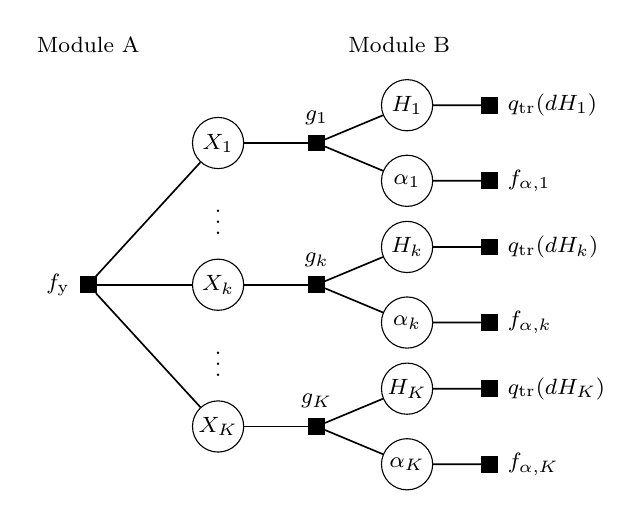
\begin{tikzpicture}[
 font=\footnotesize,
 fgvariable/.style={circle,draw,minimum size=6.5mm,inner sep=1pt},
 fgfactor/.style={rectangle,draw,fill=black,minimum size=2mm,inner sep=0pt},
 fgedge/.style={semithick}]
 \node[fgfactor,label=left:{$f_{\rm y}$}] (fy) at (0,0) {};
 \node[align=center] at (0,3.05) {Module A};
 \node[align=center] at (3.95,3.05) {Module B};
 \foreach \idx/\row in {1/1.8,k/0,K/-1.8} {
   \node[fgvariable] (x\idx) at (1.65,\row) {$X_{\idx}$};
   \node[fgfactor,label=above:{$g_{\idx}$}] (g\idx) at (2.9,\row) {};
   \node[fgvariable] (h\idx) at (4.05,{\row+0.48}) {$H_{\idx}$};
   \node[fgvariable] (a\idx) at (4.05,{\row-0.48}) {$\alpha_{\idx}$};
   \node[fgfactor,label=right:{$q_{\rm tr}(dH_{\idx})$}]
       (ph\idx) at (5.1,{\row+0.48}) {};
   \node[fgfactor,label=right:{$f_{\alpha,\idx}$}]
       (pa\idx) at (5.1,{\row-0.48}) {};
   \draw[fgedge] (fy) -- (x\idx);
   \draw[fgedge] (x\idx) -- (g\idx);
   \draw[fgedge] (g\idx) -- (h\idx) -- (ph\idx);
   \draw[fgedge] (g\idx) -- (a\idx) -- (pa\idx);
 }
 \node at (1.65,0.9) {$\vdots$};
 \node at (1.65,-0.9) {$\vdots$};
\end{tikzpicture}
\caption{Factor graph of \eqref{eq:working-posterior}, with the
observation factors grouped into $f_{\rm y}$. Circles denote variable
nodes and filled squares denote factor nodes. Each $X_k$ or $H_k$
node contains $D$ complex coefficients. The likelihood couples the
user blocks, while $g_k$ imposes $X_k=\alpha_kH_k$.}
\label{fig:twc-factor-graph}
\end{figure}


Following \cite{cai2026}, module A groups $f_{\rm y}$ for column-wise
linear estimation, while module B groups the user constraints and
priors for channel and activity denoising. Conditioned on the messages
from A, the factors in B separate over users, whose blocks are obtained
by \eqref{eq:mmv-indexing}. The modules exchange Gaussian extrinsic
messages \cite{minka2001,cai2026}, denoted by
$\mathcal M_{\rm A\to B}^{(\ell)}$ and
$\mathcal M_{\rm B\to A}^{(\ell)}$ at layer $\ell$. Each module
combines its factors with the incoming message to form a local belief,
then divides its Gaussian approximation by that message to remove
the incoming contribution, following the flow in
Fig.~\ref{fig:twc-receiver}.

\begin{figure*}[t]
\centering
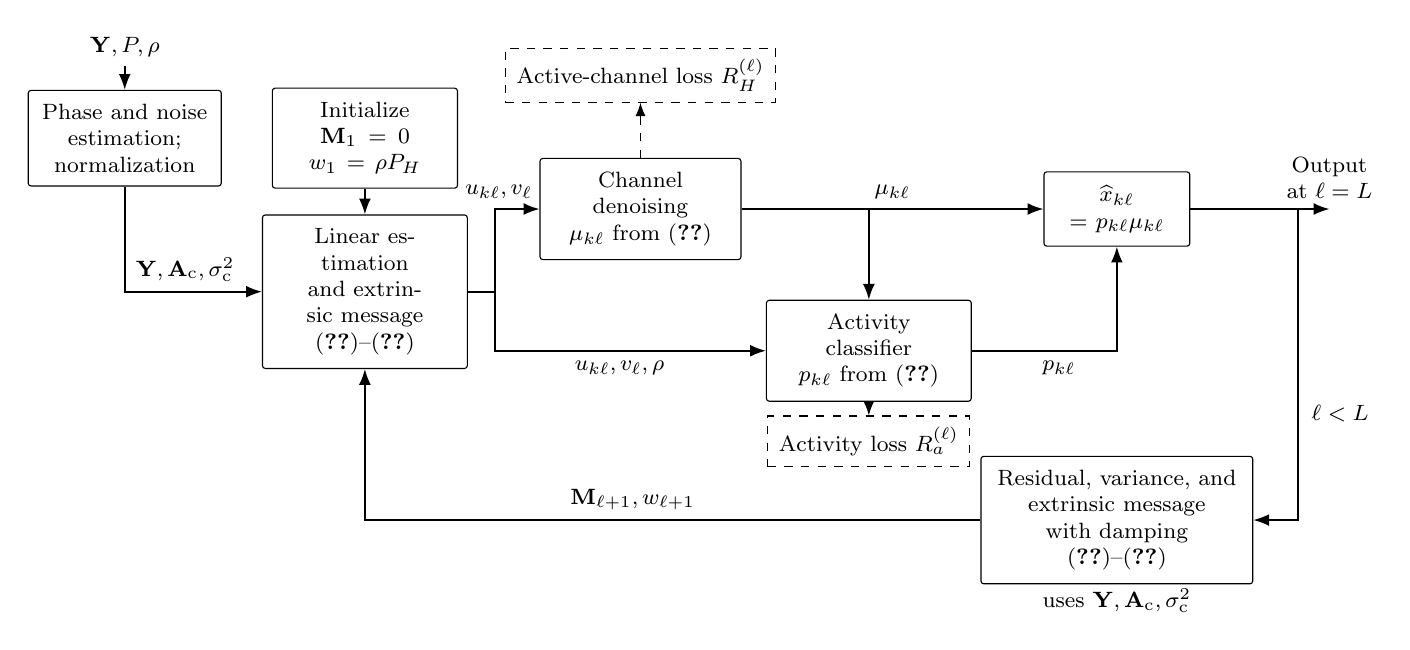
\begin{tikzpicture}[
 font=\footnotesize,
 block/.style={draw,rounded corners=1pt,align=center,
               minimum height=0.85cm,inner sep=5pt},
 flow/.style={-{Latex[length=2mm]},semithick},
 supervision/.style={-{Latex[length=1.7mm]},dashed},
 loss/.style={draw,dashed,align=center,inner sep=4pt}]
 \node[block,text width=2.1cm] (front) at (1.2,2.7)
 {Phase and noise\\estimation; normalization};
 \node[above=3mm of front] (obs) {$\mathbf Y,P,\rho$};
 \node[block,text width=2.0cm] (init) at (4.25,2.7)
 {Initialize\\$\mathbf M_1=0$\\$w_1=\rho P_H$};
 \node[block,text width=2.25cm] (linear) at (4.25,0.75)
 {Linear estimation\\and extrinsic message\\\eqref{eq:twc-linear-correction}--\eqref{eq:twc-query-calibrated}};
 \node[block,text width=2.2cm] (score) at (7.75,1.8)
 {Channel denoising\\$\mu_{k\ell}$ from \eqref{eq:twc-conditional-mean}};
 \node[block,text width=2.25cm] (activity) at (10.65,0)
 {Activity classifier\\$p_{k\ell}$ from \eqref{eq:twc-activity}};
 \node[block,text width=1.5cm] (product) at (13.8,1.8)
 {$\widehat x_{k\ell}$\\$=p_{k\ell}\mu_{k\ell}$};
 \node[block,text width=3.1cm] (feedback) at (13.8,-2.15)
 {Residual, variance, and\\extrinsic message with damping\\\eqref{eq:twc-residual-scale}--\eqref{eq:twc-damping}};
 \node[loss] (lossH) at (7.75,3.5)
 {Active-channel loss $R_H^{(\ell)}$};
 \node[loss] (lossA) at (10.65,-1.15)
 {Activity loss $R_a^{(\ell)}$};
 \draw[flow] (obs) -- (front);
 \draw[flow] (front.south) |- node[pos=0.72,above]
 {$\mathbf Y,\mathbf A_{\rm c},\sigma_{\rm c}^2$} (linear.west);
 \draw[flow] (init) -- (linear);
 \coordinate (split) at (5.9,0.75);
 \draw[flow] (linear.east) -- (split) |- (score.west);
 \draw[flow] (split) |- node[pos=0.73,below] {$u_{k\ell},v_\ell,\rho$}
 (activity.west);
 \node[above] at (5.95,1.8) {$u_{k\ell},v_\ell$};
 \draw[flow] (score.east) -- node[above] {$\mu_{k\ell}$} (product.west);
 \draw[flow] (10.65,1.8) -- (activity.north);
 \draw[flow] (activity.east) -| node[pos=0.3,below] {$p_{k\ell}$}
 (product.south);
 \draw[flow] (product.east) -- (16.5,1.8)
 node[above,align=center] {Output\\at $\ell=L$};
 \draw[flow] (16.1,1.8) |- (feedback.east);
 \node[right,align=left] at (16.15,-0.8) {$\ell<L$};
 \draw[flow] (feedback.west) -- (4.25,-2.15) -- (linear.south);
 \node[above] at (7.65,-2.15) {$\mathbf M_{\ell+1},w_{\ell+1}$};
 \node[below,align=center] at (13.8,-2.9)
 {uses $\mathbf Y,\mathbf A_{\rm c},\sigma_{\rm c}^2$};
 \draw[supervision] (score) -- (lossH);
 \draw[supervision] (activity) -- (lossA);
\end{tikzpicture}
\caption{Receiver message flow. User estimates are assembled before
the residual is computed; feedback also uses the current messages
$\mathbf R_\ell,v_\ell,\mathbf M_\ell,w_\ell$.
Dashed connections denote training losses, whose gradients propagate
through the networks and inter-layer messages.}
\label{fig:twc-receiver}
\end{figure*}

\subsection{Linear Estimation}

At layer $\ell$, the input Gaussian messages have means collected in
$\mathbf M_\ell$ and a common covariance $w_\ell\I_J$ for each
column of $\mathbf X$. Let $\mathbf m_{\ell c}$ be column $c$ of
$\mathbf M_\ell$. The input message and the belief at $f_{\rm y}$
are
\begin{equation}
 \begin{aligned}
 \mathcal M_{\rm B\to A}^{(\ell)}(\mathbf X)
 &=\prod_{c=1}^{C}\CN(\mathbf x_c;
                  \mathbf m_{\ell c},w_\ell\I_J),\\
 b_{\rm A}^{(\ell)}(\mathbf X)
 &\propto f_{\rm y}(\mathbf X)
             \mathcal M_{\rm B\to A}^{(\ell)}(\mathbf X).
 \end{aligned}
 \label{eq:twc-linear-belief}
\end{equation}
Completing the square in \eqref{eq:twc-linear-belief} gives the mean
$\mathbf M_\ell+\bm\Delta_\ell$ and average marginal variance
$t_\ell$, where
\begin{equation}
 \begin{aligned}
 \bm\Delta_\ell&=w_\ell\mathbf A_{\rm c}^{\mathsf H}
 (\sigma_{\rm c}^2\I_Q+w_\ell\mathbf A_{\rm c}\mathbf A_{\rm c}^{\mathsf H})^{-1}
 (\mathbf Y-\mathbf A_{\rm c}\mathbf M_\ell),
 \\
 t_\ell&=\frac1J\tr\!\left[
 \left(w_\ell^{-1}\I_J+
 \frac{\mathbf A_{\rm c}^{\mathsf H}\mathbf A_{\rm c}}{\sigma_{\rm c}^2}
 \right)^{-1}\right].
 \end{aligned}
 \label{eq:twc-linear-correction}
\end{equation}
Matching these moments gives a Gaussian approximation
$\widehat b_{\rm A}^{(\ell)}$ with covariance $t_\ell\I_J$ per
column, whose quotient with $\mathcal M_{\rm B\to A}^{(\ell)}$
gives the extrinsic variance and mean \cite{minka2001,cai2026}:
\begin{equation}
 \begin{aligned}
 v_\ell^{(0)}&=(t_\ell^{-1}-w_\ell^{-1})^{-1},\\
 \mathbf R_\ell^{(0)}&=v_\ell^{(0)}
 \left(\frac{\mathbf M_\ell+\bm\Delta_\ell}{t_\ell}
       -\frac{\mathbf M_\ell}{w_\ell}\right).
 \end{aligned}
 \label{eq:twc-linear-extrinsic}
\end{equation}
Because the Gaussian quotient links the mean and variance, we adjust
both when introducing the trainable scale
$\gamma_\ell=e^{c_{\gamma,\ell}}>0$. With
$v_\ell=\gamma_\ell v_\ell^{(0)}$, requiring the product of the
incoming and outgoing messages to retain mean
$\mathbf M_\ell+\bm\Delta_\ell$ gives
$(v_\ell\mathbf M_\ell+w_\ell\mathbf R_\ell)/(w_\ell+v_\ell)
=\mathbf M_\ell+\bm\Delta_\ell$, and hence
\begin{equation}
 v_\ell=\gamma_\ell v_\ell^{(0)},\qquad
 \mathbf R_\ell=\mathbf M_\ell+
 \left(1+\frac{v_\ell}{w_\ell}\right)\bm\Delta_\ell.
 \label{eq:twc-query-calibrated}
\end{equation}
The pair $(\mathbf R_\ell,v_\ell)$ is passed to module B, reducing
to \eqref{eq:twc-linear-extrinsic} when $\gamma_\ell=1$.

\subsection{Channel and Activity Denoising}

Rearrange $\mathbf R_\ell$ into user blocks according to
\eqref{eq:mmv-indexing}, and let $r_{k\ell}\in\mathbb C^D$ be the
vectorized block for user $k$. The Gaussian message passed to module B
is
\begin{equation}
 \mathcal M_{\rm A\to B}^{(\ell)}(\mathbf X)
 =\prod_{k=1}^{K}\CN\!\left(\vect(X_k);
                       r_{k\ell},v_\ell\I_D\right).
 \label{eq:twc-denoiser-message}
\end{equation}
At $g_k$, the constraint $X_k=\alpha_kH_k$ gives the likelihood
$\CN(r;\alpha h,v\I_D)$, where we omit the user and layer indices
and write $h=\vect(H_k)$ and $r=r_{k\ell}$. Integrating over the
channel under each activity hypothesis gives
\begin{equation}
 \begin{aligned}
 q_0(r;v)&=\CN(r;0,v\I_D),\\
 q_1(r;v)&=\int\CN(r;h,v\I_D)\,q_{\rm tr}(dh).
 \end{aligned}
 \label{eq:twc-local-densities}
\end{equation}
Multiplying by the activity prior $f_{\alpha,k}$ and normalizing
gives the joint channel and activity belief
\begin{equation}
 \begin{gathered}
 q(dh,a\mid r,v)=
 \frac{\rho^a(1-\rho)^{1-a}\CN(r;ah,v\I_D)\,q_{\rm tr}(dh)}
 {(1-\rho)q_0(r;v)+\rho q_1(r;v)},\\
 a\in\{0,1\}.
 \end{gathered}
 \label{eq:twc-local-posterior}
\end{equation}
Conditioning \eqref{eq:twc-local-posterior} on the active hypothesis
gives the conditional channel mean
\begin{equation}
 \mu^\star(r,v)=\E[h\mid r,\alpha=1]
 =\frac{\int h\,\CN(r;h,v\I_D)\,q_{\rm tr}(dh)}{q_1(r;v)}.
 \label{eq:twc-local-channel-target}
\end{equation}
The activity probability follows from Bayes' rule as
\begin{equation}
 p^\star(r,v)=\Pr(\alpha=1\mid r)
 =\frac{\rho q_1(r;v)}
 {(1-\rho)q_0(r;v)+\rho q_1(r;v)}.
 \label{eq:twc-local-activity-target}
\end{equation}
Since $x=\alpha h$ vanishes under the inactive hypothesis, averaging
over the two activity states gives \cite{cai2026}
\begin{equation}
 \E[x\mid r]=p^\star(r,v)\mu^\star(r,v).
 \label{eq:twc-mixture-mean}
\end{equation}
Evaluating $\mu^\star$ and $p^\star$ requires integration over the
$D$-dimensional channel distribution for every user and layer, so we
approximate them with a score-based denoiser and an activity classifier.

Let $u_{k\ell}\in\mathbb R^{2D}$ denote the real and imaginary parts
of the denoiser input for user $k$. Based on the score representation developed
in Section~\ref{sec:learning}, the channel estimate is
\begin{equation}
 \mu_{k\ell}=u_{k\ell}
       +a_\ell\frac{v_\ell}{2}s_{\theta_\ell}(u_{k\ell},v_\ell),
 \qquad a_\ell=e^{c_{\alpha,\ell}}.
 \label{eq:twc-conditional-mean}
\end{equation}
Here $s_{\theta_\ell}$ is the score network in layer $\ell$,
$v_\ell/2$ is the noise variance per real coordinate, and $a_\ell$
controls the denoising correction.

For the classifier, rewriting \eqref{eq:twc-local-activity-target}
in terms of posterior odds gives
\begin{equation}
 \logit p^\star(r,v)
 =\logit(\rho)+\log\frac{q_1(r;v)}{q_0(r;v)}.
 \label{eq:twc-activity-odds}
\end{equation}
Representing the likelihood-ratio term by a trainable log-odds
correction \cite{menon2016}, the classifier uses the input and
conditional channel estimate to compute
\begin{equation}
 p_{k\ell}=\sigmoid\!\left(\logit(\rho)+
 g_{\phi_\ell}(u_{k\ell},v_\ell,\mu_{k\ell},\rho)\right),
 \label{eq:twc-activity}
\end{equation}
where $\phi_\ell$ denotes the classifier parameters.
Substituting the channel and activity estimates into
\eqref{eq:twc-mixture-mean} gives
\begin{equation}
 \widehat x_{k\ell}=p_{k\ell}\mu_{k\ell}.
 \label{eq:twc-estimate}
\end{equation}
The estimates form $\widehat{\mathbf X}_\ell$ after conversion to
complex form and rearrangement by \eqref{eq:mmv-indexing}.
All users share the networks within a layer, with soft probabilities
retained until the final activity decision.

\subsection{Extrinsic Message Update}

To form the Gaussian return message, we associate
$\widehat{\mathbf X}_\ell$ with a common scalar variance, which we
estimate from the observation residual. Under the fixed-parameter
model, a zero-mean error with covariance $\tau\I_J$
per column and uncorrelated with the noise would satisfy
\[
 \E\|\mathbf Y-\mathbf A_{\rm c}\widehat{\mathbf X}_\ell\|_F^2
 =C\tau\|\mathbf A_{\rm c}\|_F^2+QC\sigma_{\rm c}^2.
\]
This relation motivates the normalized residual quantity
\begin{equation}
 e_\ell=\frac{\|\mathbf Y-\mathbf A_{\rm c}\widehat{\mathbf X}_\ell\|_F^2
                   -QC\sigma_{\rm c}^2}
                  {C\|\mathbf A_{\rm c}\|_F^2}.
 \label{eq:twc-residual-scale}
\end{equation}
To keep the return variance positive, we map $e_\ell$ to a ratio
$q_\ell\in(0,1)$ with a trainable scale:
\begin{equation}
 \begin{aligned}
 z_\ell&=e^{c_{\beta,\ell}}
 \left[\eta v_\ell\operatorname{softplus}
       \!\left(\frac{e_\ell}{\eta v_\ell}\right)+\epsilon_s\right],\\
 q_\ell&=\epsilon_r+(q_{\max}-\epsilon_r)
 \tanh\!\left(\frac{z_\ell}{(q_{\max}-\epsilon_r)v_\ell}\right),
 \end{aligned}
 \label{eq:twc-feedback-ratio}
\end{equation}
where $\operatorname{softplus}(x)=\log(1+e^x)$,
$\eta,\epsilon_s>0$, and $0<\epsilon_r<q_{\max}<1$ are fixed.
The softplus handles negative residual values, while
$\epsilon_r<q_\ell<q_{\max}$ keeps the output variance
$v_\ell q_\ell$ below $v_\ell$, giving positive extrinsic precision.
With $\widehat{\mathbf x}_{\ell c}$ denoting column $c$ of
$\widehat{\mathbf X}_\ell$, the Gaussian output and return message are
\begin{equation}
 \begin{aligned}
 \widehat b_{\rm B}^{(\ell)}(\mathbf X)
 &=\prod_{c=1}^{C}\CN(\mathbf x_c;
       \widehat{\mathbf x}_{\ell c},v_\ell q_\ell\I_J),\\
 \widetilde{\mathcal M}_{\rm B\to A}^{(\ell+1)}(\mathbf X)
 &\propto\frac{\widehat b_{\rm B}^{(\ell)}(\mathbf X)}
                 {\mathcal M_{\rm A\to B}^{(\ell)}(\mathbf X)}.
 \end{aligned}
 \label{eq:twc-feedback-message}
\end{equation}
Evaluating this Gaussian quotient gives
\begin{equation}
 \widetilde{\mathbf M}_{\ell+1}
 =\frac{\widehat{\mathbf X}_\ell-q_\ell\mathbf R_\ell}{1-q_\ell},
 \qquad
 \widetilde w_{\ell+1}=\frac{v_\ell q_\ell}{1-q_\ell}.
 \label{eq:twc-feedback-proposal}
\end{equation}
We damp the resulting message in its natural parameters
\cite{vehtari2020}:
\begin{equation}
 \begin{aligned}
 w_{\ell+1}^{-1}&=(1-\delta_\ell)w_\ell^{-1}
                    +\delta_\ell\widetilde w_{\ell+1}^{-1},\\
 \frac{\mathbf M_{\ell+1}}{w_{\ell+1}}
 &=(1-\delta_\ell)\frac{\mathbf M_\ell}{w_\ell}
       +\delta_\ell\frac{\widetilde{\mathbf M}_{\ell+1}}
                           {\widetilde w_{\ell+1}}.
 \end{aligned}
 \label{eq:twc-damping}
\end{equation}
Here $\delta_\ell=\min\{1,w_{\rm ref}/\widetilde w_{\ell+1}\}$
and $w_{\rm ref}=\rho P_H$, with
$P_H=\E_{q_{\rm tr}}\|h\|^2/D$ denoting the average channel power
per coefficient.
Messages with variance above the prior value $w_{\rm ref}$ receive
less weight, while averaging positive precisions preserves a positive
variance. The resulting $(\mathbf M_{\ell+1},w_{\ell+1})$ defines
$\mathcal M_{\rm B\to A}^{(\ell+1)}$ in
\eqref{eq:twc-linear-belief}, completing the layer update.

\section{Score Pretraining and Joint Receiver Training}
\label{sec:learning}

We first learn the channel score from perturbed channel samples and
then train the unfolded receiver on received pilots, jointly adapting
the channel denoisers, activity classifiers, and message parameters.

\subsection{First-Order Score Matching}

For a normalized channel sample $h_R\in\mathbb R^{2D}$, we form
the perturbed observation $u=h_R+\sqrt{v/2}\,\varepsilon$, where
$\varepsilon\sim\mathcal N(0,\I_{2D})$. Denote the perturbed
density, the real-coordinate form of $q_1$ in
\eqref{eq:twc-local-densities}, by $q_{1,R}(u;v)$ and its score by
$s^\star(u,v)=\nabla_u\log q_{1,R}(u;v)$.
Tweedie's formula relates this score to the conditional channel mean
\cite{efron2011,cai2026}:
\begin{equation}
\E[h_R\mid u]=u+\frac v2\,s^\star(u,v).
 \label{eq:twc-tweedie}
\end{equation}
Replacing $s^\star$ by a score network gives the denoiser in
\eqref{eq:twc-conditional-mean}, initially with $a_\ell=1$, without
direct integration over the channel distribution. To learn the
unknown marginal score, denoising score matching uses the Gaussian
perturbation score $-\varepsilon/\sqrt{v/2}$ as the training target
while preserving the score-matching minimizers
\cite{vincent2011,song2019}. With variance weighting, the loss is
\begin{equation}
 \mathcal L_{\rm DSM}(\theta)=\E_{h_R,v,\varepsilon}
 \left[\frac{\|\sqrt{v/2}\,s_\theta(h_R+\sqrt{v/2}\varepsilon,v)
                      +\varepsilon\|^2}{2D}\right].
 \label{eq:twc-dsm}
\end{equation}
Samples are drawn before activity masking and perturbed over a range
of noise levels, with continuous delays and Doppler shifts represented
in their effective-channel coefficients. The learned score supplies
the conditional channel mean under the active hypothesis; activity
probabilities are learned from received pilots in the next stage.

\subsection{Joint Channel and Activity Training}
\label{sec:twc-joint-training}

To adapt the pretrained denoisers to their layer inputs, each
training observation passes through the updates in
Section~\ref{sec:algorithm}, using the sensing matrix and noise variance
supplied by the physical model. The trainable parameters are
$\theta_\ell$, $\phi_\ell$, $c_{\alpha,\ell}$, $c_{\gamma,\ell}$,
and, for layers that return a message, $c_{\beta,\ell}$.
For a fixed distribution of denoiser inputs, expected squared error on
active users and expected binary cross-entropy on all users are minimized by the
conditional channel mean and activity probability, respectively
\cite{menon2016}, matching the two targets in
\eqref{eq:twc-mixture-mean}.

Suppose the receiver training set contains $B$ scenes, with $K_i$
candidate users in scene $i$. Let $h_{ik,R}$ and $\alpha_{ik}$
denote the channel and activity label of user $k$ in scene $i$.
Training and validation use disjoint physical scenes.
The channel and activity losses at layer $\ell$ are respectively
given by
\begin{align}
 R_H^{(\ell)}&=\frac{1}{E_{\rm tr}}\sum_{i,k}
       \alpha_{ik}\|\mu_{ik\ell}-h_{ik,R}\|^2,
 \label{eq:twc-channel-loss}\\
 R_a^{(\ell)}&=-\frac{1}{T_{\rm tr}}\sum_{i,k}
       \left[\alpha_{ik}\log p_{ik\ell}
       +(1-\alpha_{ik})\log(1-p_{ik\ell})\right].
 \label{eq:twc-activity-loss}
\end{align}
Here $E_{\rm tr}=\sum_{i,k}\alpha_{ik}\|h_{ik,R}\|^2$ and
$T_{\rm tr}=\sum_i K_i$ are the training set's active-channel energy
and user count, which are held fixed so that scenes with different
numbers of users retain the same normalization. The two normalized
losses receive equal coefficients in both training and model selection.

For a receiver with $m$ layers, the joint training objective is
\begin{equation}
 J_m=\frac{\sum_{\ell=1}^{m}\omega_\ell
                  \left(R_H^{(\ell)}+R_a^{(\ell)}\right)}
                 {\sum_{\ell=1}^{m}\omega_\ell},
 \label{eq:twc-layer-objective}
\end{equation}
where $\omega_\ell$ weights the loss at layer $\ell$, including
intermediate estimates used to form subsequent messages. Since the
classifier takes $\mu_{k\ell}$ as an input, gradients from the activity
loss update the channel denoiser within the same layer. Across layers,
the product $p_{k\ell}\mu_{k\ell}$ determines the residual and return
message, through which later channel losses update earlier activity
classifiers and message parameters. Joint training thus accounts for
both the current estimation errors and their effects on later layers.

\subsection{Progressive Training}

Each newly added layer has independent parameters and receives the
messages produced by the preceding layers. Its score network is
initialized from the same pretrained network, while its log-odds
correction $g_{\phi_\ell}$ and $c_{\alpha,\ell}$, $c_{\beta,\ell}$,
and $c_{\gamma,\ell}$ start at zero, giving an initial activity
probability of $\rho$.
Earlier layers retain their selected parameters.

At depth $m$, we first train the new layer with the earlier parameters
fixed, except for $c_{\beta,m-1}$ when $m>1$, since the preceding
layer's return message first contributes to the loss when layer $m$
is added. We then fine-tune all layers jointly at a reduced learning
rate, with both stages minimizing \eqref{eq:twc-layer-objective}.
The checkpoint minimizing the validation sum $R_H^{(m)}+R_a^{(m)}$,
using the training normalization constants, initializes the next
depth; after depth $L$, the selected parameters are fixed for inference.

\subsection{Network Structure and Inputs}

Each user's real and imaginary antenna maps form $2M$ feature channels
over the $N\times N$ input and output DAFT coordinates, allowing
convolutions to learn dependencies across antennas and coefficients
affected by continuous delays and Doppler shifts. The score network
uses conditional RefineNet \cite{cai2026,song2019}, with the structure
in Table~\ref{tab:twc-networks}. Two fully connected layers embed
$\log(v_\ell)/5$ into 64 features, from which each conditional
normalization layer obtains three coefficients per channel: a weight
for the normalized channel means added to the normalized features,
and a scale and shift for the result.

The classifier combines the denoiser input and conditional channel
estimate into $4M$ channels, scaled by $(1+v_\ell)^{-1/2}$, and
processes them with the convolutions and pooling in
Table~\ref{tab:twc-networks}. Its fully connected layers combine the
pooled features with
\begin{equation}
 \begin{aligned}
 \Big(&\log v_\ell,\
 \log\!\left(1+\frac{\|u_{k\ell}\|^2}{Dv_\ell}\right),\
 \log\!\left(1+\frac{\|\mu_{k\ell}\|^2}{Dv_\ell}\right),\\
 &\log\!\left(1+\frac{\|u_{k\ell}-\mu_{k\ell}\|^2}{Dv_\ell}\right),\
 \logit\rho\Big)
 \end{aligned}
 \label{eq:twc-classifier-features}
\end{equation}
to produce the log-odds correction in \eqref{eq:twc-activity}.
These energy terms describe the input, channel estimate, and residual
relative to the noise level. Since both networks act on individual
users with shared parameters within a layer, their input dimensions
depend on $M$ and $N$, whereas $K$ determines the number of evaluations
and $Q$ enters through the linear estimator.

\begin{table}[t]
\centering
\caption{Network structure for $M=N=16$. Tensor sizes are feature
channels $\times$ height $\times$ width.}
\label{tab:twc-networks}
\footnotesize
\setlength{\tabcolsep}{3pt}
\begin{tabular}{>{\raggedright\arraybackslash}p{0.43\linewidth}
                >{\raggedright\arraybackslash}p{0.49\linewidth}}
\toprule
Stage & Output size or operation\\
\midrule
\multicolumn{2}{l}{\textit{Score network}}\\
Input & $32\times16\times16$; affine map $2u-1$\\
Input convolution, $3\times3$ & $128\times16\times16$\\
Residual groups 1 and 2 & $128\times16\times16$; $256\times8\times8$\\
Residual groups 3 and 4 & $256\times8\times8$ each; dilation 2 and 4\\
Four refinement blocks & Widths 256, 256, 128, 128; final size $16\times16$\\
Output & Conditional normalization, ELU, $3\times3$ convolution; divide by $\sqrt{v/2}$\\
\midrule
\multicolumn{2}{l}{\textit{Activity classifier}}\\
Input & $64\times16\times16$; divide by $\sqrt{1+v}$\\
Three $3\times3$ convolutions & $32\times16\times16$, $64\times8\times8$, $64\times4\times4$\\
Spatial average pooling & 64 features\\
Concatenation & 64 features and the five scalars in \eqref{eq:twc-classifier-features}\\
Two fully connected layers & $69\rightarrow64\rightarrow1$\\
\bottomrule
\end{tabular}
\par\smallskip
\begin{minipage}{0.95\linewidth}
\footnotesize
Each score residual group contains two blocks. Refinement uses
skip connections and bilinear interpolation when sizes differ.
The score network uses exponential linear units (ELUs), while its
noise-conditioning layers and the activity hidden layers use
$x\sigmoid(x)$.
\end{minipage}
\end{table}

\section{Overall Algorithm}
\label{sec:overall}

\subsection{Message Scheduling}

The receiver first estimates the phase increments and noise variance
as described in Appendix~\ref{app:frontend}, after which the resulting
$\mathbf A_{\rm c}$ and $\sigma_{\rm c}^2$ remain fixed throughout
the $L$ unfolded layers. Although the phase fit uses one dominant
path per candidate terminal, the denoisers recover the full multipath
channel. Table~\ref{tab:twc-algorithm} summarizes the complete receiver,
where $\widehat H_{k,L}$ denotes the complex channel tensor obtained
from $\mu_{kL}$ and the final channel outputs are restored to their
original scale.

\begin{table}[t]
\centering
\caption{Deep-unfolded MP receiver with a score-based channel prior for JADCE}
\label{tab:twc-algorithm}
\begin{tabular}{p{0.93\linewidth}}
\toprule
\textbf{Input:} received pilots $\mathbf Y$, original pilot tensor $P$,
activity probability $\rho$, trained layer parameters, normalization
factor $s$, and average channel power $P_H$.\\
\textbf{Preprocessing:} estimate $\widehat\sigma^2$ and
$\widehat{\bm\beta}$ by Appendix~\ref{app:frontend}; construct
$\mathbf A_{\rm c}=\widehat{\mathbf A}$.
Normalize $\mathbf Y$ and $\widehat\sigma^2$ by $s$ and $s^2$,
and set $\sigma_{\rm c}^2$ to the normalized noise estimate.\\
\textbf{Initialize:} set $\mathbf M_1=\mathbf0$ and
$w_1=w_{\rm ref}=\rho P_H$, and compute a thin singular value
decomposition of $\mathbf A_{\rm c}$.\\
\textbf{For} $\ell=1,\ldots,L$:\\
1. Compute the linear update and the mean and variance passed to the denoiser using
\eqref{eq:twc-linear-correction}--\eqref{eq:twc-query-calibrated}.\\
2. Estimate the channels and activity probabilities, and combine
them using \eqref{eq:twc-conditional-mean}, \eqref{eq:twc-activity},
and \eqref{eq:twc-estimate}.\\
3. If $\ell<L$, form the feedback message and damp it using
\eqref{eq:twc-residual-scale}--\eqref{eq:twc-damping}.\\
\textbf{Return:} $\widehat H_k^{\rm out}=s\widehat H_{k,L}$,
$\widehat X_k^{\rm out}=s p_{kL}\widehat H_{k,L}$,
$\widehat\alpha_k=\mathbf1\{p_{kL}\geq1/2\}$, and $p_{kL}$.\\
\bottomrule
\end{tabular}
\end{table}

\subsection{Computational Complexity Analysis}

Since $\mathbf A_{\rm c}$ is fixed, one thin singular value decomposition
(SVD), at cost $O(QJr)$ with $J=KN$, $C=MN$, and $r=\min(Q,J)$,
suffices to evaluate the general linear estimator in
\eqref{eq:twc-linear-correction} across all layers. Computing the
residuals and applying the singular vectors then cost $O(QJC)$ and
$O((Q+J)rC)$ per layer, respectively. Denoting the costs of one user's
score network and activity classifier in Table~\ref{tab:twc-networks}
by $F_s$ and $F_a$, we obtain
\begin{equation}
 C_{\rm layer}=O\left(QJC+(Q+J)rC+K(F_s+F_a)\right).
 \label{eq:twc-layer-complexity}
\end{equation}
For the phase estimator, let $G_{\rm c}$ be the number of coarse
delay--Doppler path matrices, $B_\phi\geq Q$ the number of phase bins,
$S_\phi$ the number of coordinate sweeps, and $E_\phi$ the number of
path-matrix evaluations for Doppler ranking and local refinement,
including derivative evaluations up to a constant factor. The costs
of precomputing the path responses, searching users by correlation and
fast Fourier transforms (FFTs), refining the paths, and jointly
refitting the gains give, for $K\leq QN$,
\begin{equation}
 \begin{aligned}
 C_{\rm phase}=O\big(&G_{\rm c}N^3+KG_{\rm c}QN^2\\
 &+(S_\phi+1)KG_{\rm c}M(QN+B_\phi\log B_\phi)\\
 &+E_\phi(N^3+QN^2+QNM)\\
 &+S_\phi(QNK^2+QNKM)\big).
 \end{aligned}
 \label{eq:twc-phase-complexity}
\end{equation}
Since phase estimation and the spatial covariance eigendecomposition
for noise estimation are performed once per block, the complete
online cost is
\begin{equation}
 O\left(C_{\rm phase}+QNM^2+M^3+QJr+L C_{\rm layer}\right).
 \label{eq:twc-complexity}
\end{equation}
For $Q\leq J$, the SVD and unfolded layers contribute
$O(Q^2J+L[QJC+K(F_s+F_a)])$, including the residual used for
variance estimation. Reducing $L$ therefore saves repeated linear
updates and network evaluations, while the front-end and SVD costs
remain fixed. With $P_s$ score-network and $P_a$ classifier parameters
per layer, the receiver stores $L(P_s+P_a+3)$ parameter scalars;
the operator, SVD, and messages require
$O(QJ+(Q+J)r+JC+QC)$ additional storage, excluding network activations
and the phase-estimation cache.

% \section{Simulation Results}
\label{sec:simulations}

% TODO: Write this section before enabling its input in main.tex.

% \section{Conclusion}
\label{sec:conclusion}

% TODO: Write this section before enabling its input in main.tex.


\appendices
\numberwithin{equation}{section}
\section{Phase and Noise Estimation}
\label{app:frontend}

\subsection{Inter-frame phase estimation}
Stack the received samples as
$[\mathbf Y_{\rm s}]_{qN+r,m}=Y_{qmr}$, so that
$\mathbf Y_{\rm s}\in\mathbb C^{QN\times M}$.
To estimate the phase increments, we approximate the contribution of each
candidate terminal by one dominant path with an unconstrained complex
gain at each antenna.
Absorbing the common scalar phase into the gain, we define the path matrix as
\begin{equation}
 \begin{aligned}
 \mathbf G_0(d,\nu)&=e^{-j2\pi c_1d^2}\mathbf G(d,\nu;0),\\
 [\mathbf h_k(d,\nu)]_{qN+r}
 &=e^{j2\pi\nu qT_{\rm frame}}
 \sum_{n=0}^{N-1}[\mathbf G_0(d,\nu)]_{rn}P_{qkn}.
 \end{aligned}
 \label{eq:phase-atom}
\end{equation}
The delay search is restricted to $d\in[0,N)$ and the Doppler search to $|\nu|\leq\nu_{\max}$. Under $2Nc_1\in\mathbb N_+$, shifting
the delay by an integer multiple of $N$ changes the path operator by
a scalar phase, which the fitted gains absorb. With
$\mathbf h_k=\mathbf h_k(d_k,\nu_k)$ and gain vector
$\mathbf b_k\in\mathbb C^M$, the fitting objective is
\begin{equation}
 \min_{\{d_k,\nu_k,\mathbf b_k\}}
 \left\|\mathbf Y_{\rm s}-\sum_{k=1}^K
 \mathbf h_k\mathbf b_k^{\mathsf T}\right\|_F^2.
 \label{eq:phase-fit}
\end{equation}
When updating terminal $k$, we fix the other contributions and define
$\mathbf Z_k=\mathbf Y_{\rm s}-\sum_{j\ne k}
\mathbf h_j\mathbf b_j^{\mathsf T}$. For a given $(d,\nu)$, the
least-squares gain and the resulting objective are given by
\begin{equation}
 \begin{aligned}
 \mathbf b_k^{\mathsf T}(d,\nu)
 &=\frac{\mathbf h_k(d,\nu)^{\mathsf H}\mathbf Z_k}
 {\|\mathbf h_k(d,\nu)\|^2},\\
 J_k(d,\nu)&=\|\mathbf Z_k\|_F^2-
 \frac{\|\mathbf h_k(d,\nu)^{\mathsf H}\mathbf Z_k\|^2}
 {\|\mathbf h_k(d,\nu)\|^2}.
 \end{aligned}
 \label{eq:phase-variable-projection}
\end{equation}
The gains are eliminated from the separable nonlinear least-squares
problem by variable projection \cite{oleary2013}. Coarse correlations over
delay, within-frame Doppler, and frame phase provide initial candidates.
A phase candidate $\beta$ corresponds to Doppler aliases
\begin{equation}
 \nu_j=\frac{\beta+2\pi j}{2\pi T_{\rm frame}},\qquad
 j\in\mathbb Z,\quad |\nu_j|\leq\nu_{\max}.
 \label{eq:phase-aliases}
\end{equation}
Candidates are ranked using the pilot response vector in
\eqref{eq:phase-atom}, which enforces the same Doppler within and across
frames. The selected candidates undergo bounded local refinement by
L-BFGS-B \cite{zhu1997}, with delay restricted to one differentiable
branch of the wrapped waveform. Each coordinate update is accepted
when it does not increase the residual energy, up to numerical tolerance.
After each sweep, all antenna gains are refitted jointly by least squares.

The receiver uses a fixed number of complete sweeps, retaining the previous
position as an additional refinement starting point after the first sweep.
It sets $\widehat\beta_k=\operatorname{wrap}
(2\pi\widehat\nu_kT_{\rm frame})$ and constructs
$\widehat{\mathbf A}$ by \eqref{eq:effective-pilot}.
This local fit provides phase estimates for all candidate terminals.
The nonlinear denoiser then estimates the full channel tensor in
\eqref{eq:channel}.

\subsection{Noise variance estimation}
Let $L=QN>M\geq2$ and form the spatial sample covariance
\begin{equation}
 \begin{aligned}
 \widehat{\mathbf R}_y&=\frac1L\sum_{q=0}^{Q-1}\sum_{r=0}^{N-1}
 \mathbf y_{qr}\mathbf y_{qr}^{\mathsf H},\\
 \mathbf y_{qr}&=(Y_{q0r},\ldots,Y_{q,M-1,r})^{\mathsf T}.
 \end{aligned}
 \label{eq:spatial-noise-covariance}
\end{equation}
Write its eigenvalues in descending order as
$\lambda_1\geq\cdots\geq\lambda_M$; values below
$\epsilon_{\rm mach}\lambda_1$ are floored at that level before
taking logarithms. For a candidate spatial signal rank $j$, define
\begin{equation}
 \bar\lambda_j=\frac1{M-j}\sum_{i=j+1}^M\lambda_i,\qquad
 \log g_j=\frac1{M-j}\sum_{i=j+1}^M\log\lambda_i.
 \label{eq:noise-tail-statistics}
\end{equation}
The Wax--Kailath minimum description length (MDL) criterion, as reviewed
in \cite{nadakuditi2008}, gives
\begin{equation}
 \begin{aligned}
 \widehat r_{\rm s}
 &=\arg\min_{0\leq j<M}\Big\{
 L(M-j)(\log\bar\lambda_j-\log g_j)\\
 &\hspace{6em}+\frac{j(2M-j)}2\log L\Big\},\\
 \widehat\sigma^2&=\bar\lambda_{\widehat r_{\rm s}}.
 \end{aligned}
 \label{eq:noise-mdl}
\end{equation}
Under a lower-rank spatial signal plus white-noise model, the criterion
selects the spatial signal rank and estimates the noise variance from
the remaining eigenvalues. Both $\widehat\sigma^2$ and
$\widehat{\mathbf A}$ remain fixed throughout the MP iterations.




\bibliographystyle{IEEEtran}
\bibliography{references}
\end{document}
